\documentclass[11pt]{article}

\usepackage[margin=1in]{geometry}
\usepackage[T1]{fontenc}
\usepackage[utf8]{inputenc}
\usepackage{lmodern}
\usepackage{microtype}
\usepackage[dvipsnames]{xcolor}
\usepackage{booktabs}
\usepackage{array}
\usepackage{longtable}
\usepackage{enumitem}
\usepackage{hyperref}
\usepackage{tikz}
\usetikzlibrary{arrows.meta, positioning, shapes.geometric, fit, calc}

\hypersetup{
  colorlinks=true,
  linkcolor=MidnightBlue,
  urlcolor=MidnightBlue
}

\setlist[itemize]{leftmargin=1.5em}
\setlist[enumerate]{leftmargin=1.5em}

\title{UC Atlas Intuition Map\\
\large Hierarchy, Groupings, Questions, and Modeling Roadmap}
\author{sfn-scrna-study workspace}
\date{Last updated: 2026-03-16}

\begin{document}
\maketitle

\section*{Why this document exists}

This is not a methods section and not yet a modeling report.
It is a visual and conceptual map for the ulcerative colitis single-cell atlas
we are using as the anchor dataset.

The point is to answer five practical questions before moving further:

\begin{enumerate}
  \item What exactly is in the dataset?
  \item What are the natural ways to group and categorize the observations?
  \item Which scientific questions live at which level of the data?
  \item What have we already learned from the foundation summaries?
  \item What modeling layers should come next, in what order?
\end{enumerate}

\section*{The dataset at a glance}

The current local UC foundation summaries establish the following:

\begin{itemize}
  \item 30 donors total
  \item 12 healthy donors and 18 UC donors
  \item 133 samples total
  \item 61 epithelial samples and 72 lamina propria samples
  \item 365{,}492 cells total
  \item 51 fine cluster labels
  \item 4 coarse cluster families
  \item 59 donor-by-location rows if we split each donor into Epi and LP views
  \item 29 donors have both Epi and LP coverage
  \item 1 donor, N661, is LP-only
\end{itemize}

\section*{Figure 1: Data hierarchy}

\begin{figure}[h!]
\centering
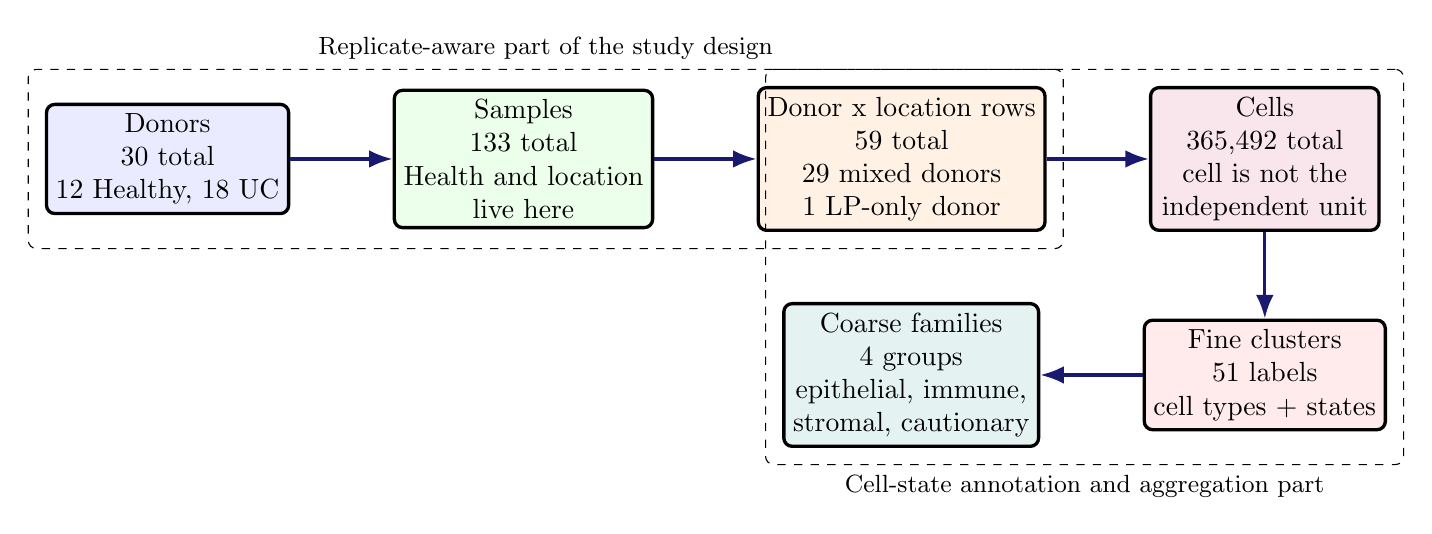
\begin{tikzpicture}[
  node distance=1.1cm and 1.3cm,
  stage/.style={draw, rounded corners=3pt, very thick, align=center, minimum width=2.9cm, minimum height=1.05cm},
  arrow/.style={-{Latex[length=3mm]}, very thick, MidnightBlue}
]
  \node[stage, fill=blue!8] (donor) {Donors\\30 total\\12 Healthy, 18 UC};
  \node[stage, fill=green!8, right=of donor] (sample) {Samples\\133 total\\Health and location\\live here};
  \node[stage, fill=orange!10, right=of sample] (locrow) {Donor x location rows\\59 total\\29 mixed donors\\1 LP-only donor};
  \node[stage, fill=purple!10, right=of locrow] (cell) {Cells\\365,492 total\\cell is not the\\independent unit};
  \node[stage, fill=red!8, below=of cell] (cluster) {Fine clusters\\51 labels\\cell types + states};
  \node[stage, fill=teal!10, left=of cluster] (family) {Coarse families\\4 groups\\epithelial, immune,\\stromal, cautionary};

  \draw[arrow] (donor) -- (sample);
  \draw[arrow] (sample) -- (locrow);
  \draw[arrow] (locrow) -- (cell);
  \draw[arrow] (cell) -- (cluster);
  \draw[arrow] (cluster) -- (family);

  \node[draw, dashed, rounded corners=3pt, fit=(donor)(sample)(locrow), inner sep=6pt, label=above:{\small Replicate-aware part of the study design}] {};
  \node[draw, dashed, rounded corners=3pt, fit=(cell)(cluster)(family), inner sep=6pt, label=below:{\small Cell-state annotation and aggregation part}] {};
\end{tikzpicture}
\caption{The same biological study can be viewed at several levels.
The critical mistake to avoid is treating the cell level as if it were the
replicate level for disease prediction.}
\end{figure}

\section*{Figure 2: How the 51 clusters should be grouped mentally}

\begin{figure}[h!]
\centering
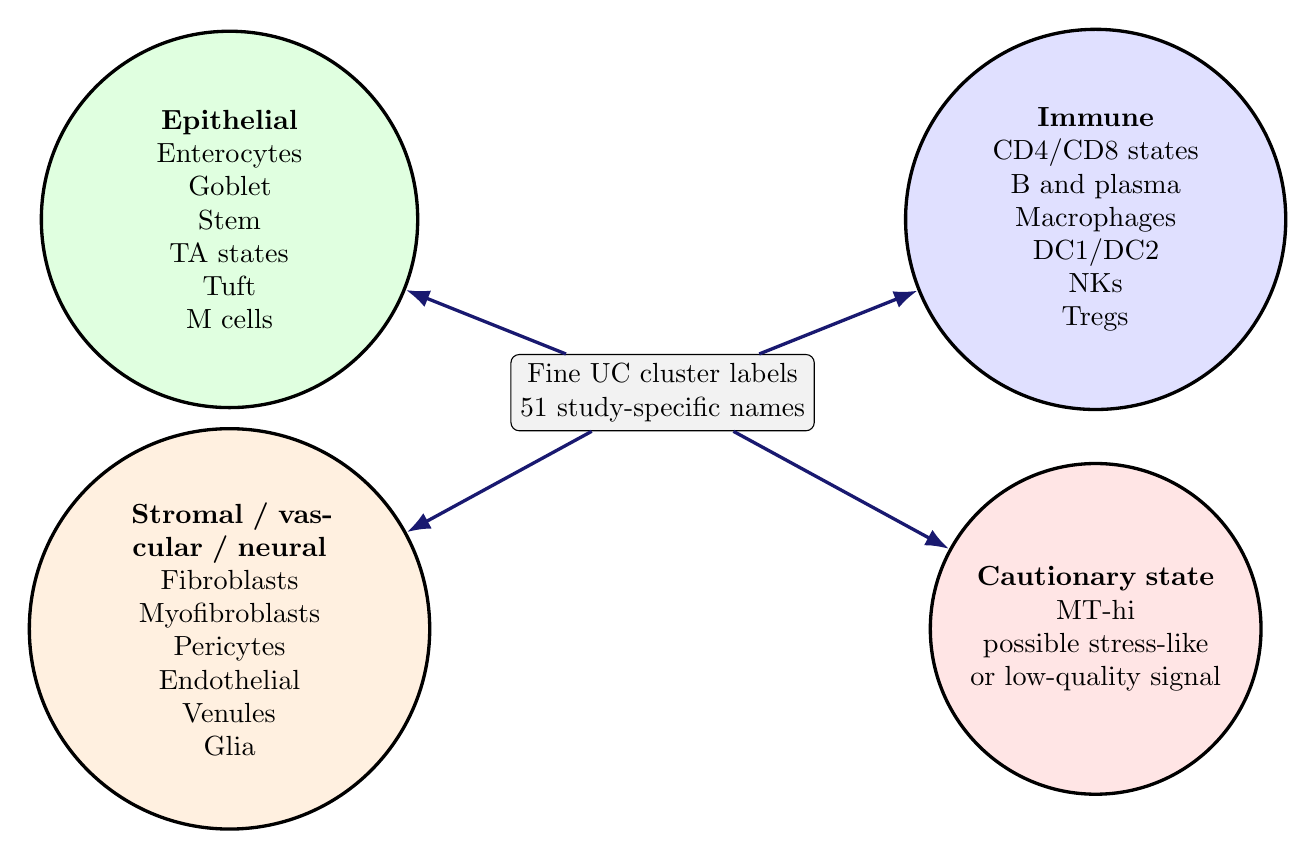
\begin{tikzpicture}[
  every node/.style={align=center},
  bubble/.style={circle, draw, very thick, minimum width=4.2cm, text width=3.5cm},
  titlebox/.style={draw, rounded corners=3pt, fill=gray!10, minimum width=3.3cm, minimum height=0.8cm}
]
  \node[titlebox] (center) at (0,0) {Fine UC cluster labels\\51 study-specific names};

  \node[bubble, fill=green!12] (epi) at (-5.5,2.2) {\textbf{Epithelial}\\
  Enterocytes\\Goblet\\Stem\\TA states\\Tuft\\M cells};

  \node[bubble, fill=blue!12] (imm) at (5.5,2.2) {\textbf{Immune}\\
  CD4/CD8 states\\B and plasma\\Macrophages\\DC1/DC2\\NKs\\Tregs};

  \node[bubble, fill=orange!12] (str) at (-5.5,-3.0) {\textbf{Stromal / vascular / neural}\\
  Fibroblasts\\Myofibroblasts\\Pericytes\\Endothelial\\Venules\\Glia};

  \node[bubble, fill=red!10] (cau) at (5.5,-3.0) {\textbf{Cautionary state}\\
  MT-hi\\
  possible stress-like\\or low-quality signal};

  \draw[-{Latex[length=3mm]}, very thick, MidnightBlue] (center) -- (epi);
  \draw[-{Latex[length=3mm]}, very thick, MidnightBlue] (center) -- (imm);
  \draw[-{Latex[length=3mm]}, very thick, MidnightBlue] (center) -- (str);
  \draw[-{Latex[length=3mm]}, very thick, MidnightBlue] (center) -- (cau);
\end{tikzpicture}
\caption{The fine cluster names mix canonical cell types, activation states,
proliferative states, and study-specific stromal subtypes.
For stable interpretation, we should usually think first at the coarse-family
level and then return to fine clusters.}
\end{figure}

\section*{What we are trying to understand}

There are several distinct questions in this dataset, and each lives at a
different level.

\begin{center}
\begin{tabular}{>{\raggedright\arraybackslash}p{2.6cm} >{\raggedright\arraybackslash}p{3.0cm} >{\raggedright\arraybackslash}p{4.0cm} >{\raggedright\arraybackslash}p{4.0cm}}
\toprule
\textbf{Question branch} & \textbf{Natural row unit} & \textbf{What it asks} & \textbf{Main risk if done badly} \\
\midrule
Atlas and annotation & Cell & What cell populations and states are present? & Over-trusting labels or mixing technical artifacts with real states \\
Composition & Donor, donor-location, or donor-by-cluster summary & Which populations expand or contract in UC? & Confusing compartment mixture with disease biology \\
Differential state & Donor by cell type or donor by location & What changes inside a cell type or compartment? & Pseudoreplication if replicate structure is ignored \\
Disease prediction & Donor or donor-location & Can Healthy vs UC be predicted honestly? & Leakage, confounding, or treating repeated rows from one donor as independent \\
\bottomrule
\end{tabular}
\end{center}

\section*{Figure 3: The question map}

\begin{figure}[h!]
\centering
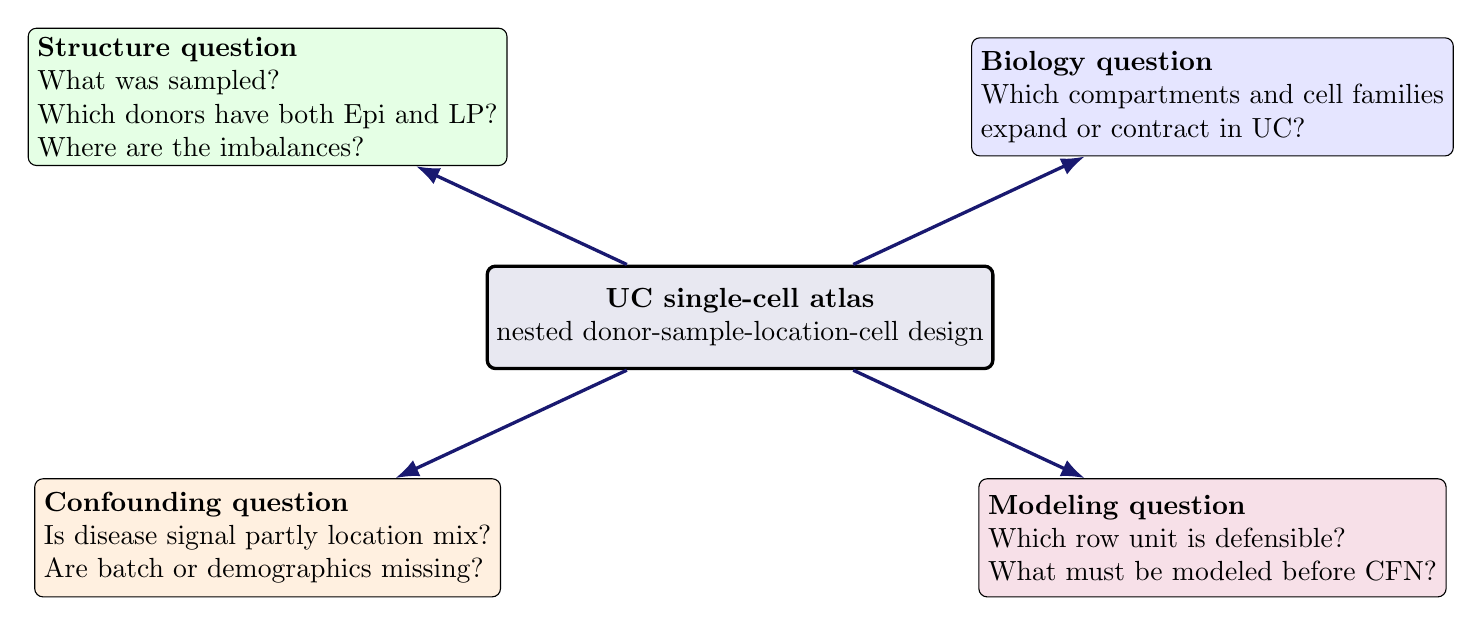
\begin{tikzpicture}[
  box/.style={draw, rounded corners=3pt, minimum width=4.2cm, minimum height=1.5cm, align=left, fill=gray!8},
  centerbox/.style={draw, very thick, rounded corners=3pt, minimum width=4cm, minimum height=1.3cm, align=center, fill=MidnightBlue!10},
  arrow/.style={-{Latex[length=3mm]}, very thick, MidnightBlue}
]
  \node[centerbox] (core) at (0,0) {\textbf{UC single-cell atlas}\\
  nested donor-sample-location-cell design};

  \node[box, fill=green!10] (structure) at (-6,2.8) {\textbf{Structure question}\\
  What was sampled?\\
  Which donors have both Epi and LP?\\
  Where are the imbalances?};

  \node[box, fill=blue!10] (biology) at (6,2.8) {\textbf{Biology question}\\
  Which compartments and cell families\\
  expand or contract in UC?};

  \node[box, fill=orange!12] (confound) at (-6,-2.8) {\textbf{Confounding question}\\
  Is disease signal partly location mix?\\
  Are batch or demographics missing?};

  \node[box, fill=purple!12] (model) at (6,-2.8) {\textbf{Modeling question}\\
  Which row unit is defensible?\\
  What must be modeled before CFN?};

  \draw[arrow] (core) -- (structure);
  \draw[arrow] (core) -- (biology);
  \draw[arrow] (core) -- (confound);
  \draw[arrow] (core) -- (model);
\end{tikzpicture}
\caption{The right workflow is not ``jump into one classifier''.
It is to answer structure, biology, confounding, and modeling questions in a
disciplined order.}
\end{figure}

\section*{What we have already learned from the current summaries}

\subsection*{1. Coarse families already shift in a coherent way}

\begin{center}
\begin{tabular}{lrrr}
\toprule
\textbf{Coarse family} & \textbf{Healthy mean} & \textbf{UC mean} & \textbf{UC - Healthy} \\
\midrule
epithelial & 0.4624 & 0.3360 & -0.1264 \\
immune & 0.4494 & 0.5475 & 0.0982 \\
stromal / vascular / neural & 0.0860 & 0.1152 & 0.0292 \\
cautionary state & 0.0022 & 0.0013 & -0.0009 \\
\bottomrule
\end{tabular}
\end{center}

This is a strong first intuition:

\begin{itemize}
  \item UC donors look less epithelial overall
  \item UC donors look more immune-rich
  \item UC donors also show more stromal and vascular support signal
\end{itemize}

This means a disease classifier may work partly because the composition
difference is real and fairly large.

\subsection*{2. Location mixture is not balanced between groups}

The donor-level location summaries show:

\begin{itemize}
  \item healthy donors have a mean LP fraction of about 0.55
  \item UC donors have a mean LP fraction of about 0.75
  \item N661 is LP-only
  \item 29 donors have both Epi and LP, so donor-by-location analysis is feasible
\end{itemize}

So donor-only all-cell pseudobulk is useful, but not enough for interpretation.
It must be followed by donor-by-location pseudobulk.

\subsection*{3. Unevenness exists at the donor level}

The donor summaries already show that UC donors are more uneven than healthy
donors in both cell count and sample count.

That matters because:

\begin{itemize}
  \item some donors contribute much more material than others
  \item donor-level summaries should remain the unit of inference
  \item technical metadata should not quietly become shortcut predictors
\end{itemize}

\section*{What counts as an ``observation'' in this project}

\begin{center}
\begin{tabular}{>{\raggedright\arraybackslash}p{2.1cm} >{\raggedright\arraybackslash}p{3.0cm} >{\raggedright\arraybackslash}p{2.4cm} >{\raggedright\arraybackslash}p{4.8cm}}
\toprule
\textbf{Level} & \textbf{Example row} & \textbf{Independent?} & \textbf{Best use} \\
\midrule
Cell & one barcode from N10.EpiA & No & annotation, clustering, cell-state discovery \\
Sample & N10.EpiA or N10.LPA & Not fully, repeated within donor & sample-level summaries, local inflammation framing \\
Donor-location & N10-Epi or N10-LP & Not fully, repeated within donor & location-aware pseudobulk and sensitivity analysis \\
Donor & N10 & Yes, this is the closest current replicate unit & disease prediction and honest cross-validation \\
Coarse family summary & epithelial proportion for N10 & Derived donor-level feature & stable biological interpretation \\
\bottomrule
\end{tabular}
\end{center}

The practical consequence is simple:

\begin{itemize}
  \item donor-level prediction can use donor or donor-location rows
  \item but train and validation must stay grouped by donor
  \item 59 donor-location rows do not mean 59 independent replicates
\end{itemize}

\section*{Figure 4: Modeling roadmap}

\begin{figure}[h!]
\centering
\begin{tikzpicture}[
  node distance=0.95cm and 1.2cm,
  step/.style={
    draw,
    rounded corners=3pt,
    minimum height=1.0cm,
    text width=0.66\linewidth,
    align=center,
    font=\small,
    inner sep=6pt
  },
  arrow/.style={-{Latex[length=3mm]}, very thick, MidnightBlue}
]
  \node[step, fill=gray!12] (f0) {Foundation audit\\
  hierarchy, labels, location, covariates};
  \node[step, fill=green!12, below=of f0] (f1) {Coarse family and cluster composition\\
  understand what is shifting};
  \node[step, fill=blue!12, below=of f1] (f2) {Donor-level all-cell pseudobulk\\
  first simple disease benchmark};
  \node[step, fill=orange!12, below=of f2] (f3) {Donor-by-location pseudobulk\\
  interpretation-safe sensitivity layer};
  \node[step, fill=purple!12, below=of f3] (f4) {Donor-by-cell-type pseudobulk\\
  richer but more granular representation};
  \node[step, fill=red!10, below=of f4] (f5) {Later extensions\\
  differential state and pathway work\\
  plus structured models only after the conventional ladder is stable};

  \draw[arrow] (f0) -- (f1);
  \draw[arrow] (f1) -- (f2);
  \draw[arrow] (f2) -- (f3);
  \draw[arrow] (f3) -- (f4);
  \draw[arrow] (f4) -- (f5);
\end{tikzpicture}
\caption{The modeling ladder we should follow from here.
The important point is that donor-by-location pseudobulk is no longer optional
for interpretation once the location imbalance is visible.}
\end{figure}

\section*{What we are trying to understand before moving forward}

\begin{enumerate}
  \item How much of the Healthy vs UC signal is simply epithelial versus LP mixture?
  \item Which changes remain visible inside Epi alone and inside LP alone?
  \item Which changes are broad family shifts, and which are fine-cluster shifts?
  \item Which later modeling claims would still hold after location-aware sensitivity analysis?
  \item What representation should later structured models be asked to improve on:
  donor-only, donor-by-location, or donor-by-cell-type?
\end{enumerate}

\section*{Immediate next actions}

\begin{enumerate}
  \item Keep using the coarse family summaries for intuitive interpretation.
  \item Build donor-by-location pseudobulk tables as the next processed artifact.
  \item Compare all-cell donor pseudobulk against Epi-only and LP-only views.
  \item Only after that, run the first baseline stack and interpret performance.
  \item Treat CFN as a later representation question, not the next thing to rush into.
\end{enumerate}

\section*{Local artifacts this map is based on}

\begin{itemize}
  \item \texttt{data/processed/uc\_scp259/exploration/foundation\_summary.txt}
  \item \texttt{data/processed/uc\_scp259/exploration/donor\_location\_overview.tsv}
  \item \texttt{data/processed/uc\_scp259/exploration/cluster\_label\_mean\_deltas.tsv}
  \item \texttt{data/processed/uc\_scp259/exploration/cluster\_family\_label\_deltas.tsv}
  \item \texttt{docs/uc\_cluster\_glossary.md}
  \item \texttt{docs/uc\_foundations\_and\_reference\_workflows.md}
\end{itemize}

\end{document}
